\documentclass{article}
%\documentclass[doc,english]{apa}
\usepackage[utf8]{inputenc}

% packages
\usepackage{amsmath,amsfonts,amssymb, bm}
\usepackage{graphicx}
\usepackage[colorlinks=true, allcolors=blue]{hyperref}
\usepackage{apacite}
\usepackage{authblk}  % for authors
\usepackage{caption}
%\usepackage{setspace} % doublespacing
\usepackage{subcaption}
\usepackage{booktabs}
\usepackage{nicefrac}

\usepackage{color}
\usepackage{todonotes}

%\usepackage{etoolbox}
%\makeatletter
%\patchcmd{\Ginclude@eps}{"#1"}{#1}{}{}
%\makeatother

\newcommand{\EJ}[1]{\todo[inline, color=green]{EJ: {#1}}}
\newcommand{\DON}[1]{\todo[inline, color=white]{Don: {#1}}}

\newcommand{\Irater}{r}
\newcommand{\Iitem}{i}
\newcommand{\Ipatient}{p}
\newcommand{\Incat}{c}

\newcommand{\Trater}{\expandafter\MakeUppercase\expandafter{\Irater}}
\newcommand{\Titem}{\expandafter\MakeUppercase\expandafter{\Iitem}}
\newcommand{\Tpatient}{\expandafter\MakeUppercase\expandafter{\Ipatient}}
\newcommand{\Tncat}{\expandafter\MakeUppercase\expandafter{\Incat}}

\newcommand{\ilogit}[1]{\text{logit}^{-1}\left(#1\right)}


\title{Cultural Consensus Theory for the Evaluation of Patients’ Behavior in Psychiatric  Detention Centers}

\renewcommand{\thefootnote}{\fnsymbol{footnote}}
\author[1]{Don van den Bergh\thanks{Correspondence concerning this article should be addressed to:  
\\  Don van den Bergh 
\\  University of Amsterdam, Department of Psychological Methods
\\  Postbus 15906, 1001 NK Amsterdam, The Netherlands
\\  E-Mail should be sent to: donvdbergh@hotmail.com.}}
\author[1]{wie nog meer?}
\author[1]{Eric-Jan Wagenmakers}
\affil[1]{University of Amsterdam}
\date{}

\begin{document}

\maketitle

\begin{abstract}
In many psychiatric detention centers, patients' mental health is monitored at regular intervals. Typically, clinicians score patients using a Likert scale on multiple criteria including hostility. Having an overview of patients’ scores benefits staff members in at least three ways. First, the scores may help adjust treatment to the individual patient; second, the change in scores over time allow an assessment of treatment effectiveness; third, the scores may warn staff that particular patients are at high risk of turning violent. Practical importance notwithstanding, current practices for the analysis of mental health scores are suboptimal: evaluations from different clinicians are averaged (as if the Likert scale were linear and the clinicians identical), and patients are analyzed in isolation (as if they were independent). Uncertainty estimates of the resulting score are often ignored. Here we outline a quantitative program for the analysis of mental health scores using cultural consensus theory (CCT; \citeNP{Anders2015cultural}). CCT models take into account the ordinal nature of the Likert scale, the individual differences among clinicians, and the possible commonalities between patients. In a simulation, we compare the predictive performance of the CCT model to the current practice of aggregating raw observations and, as a more reasonable alternative, against often-used machine learning toolboxes. In addition, we outline the substantive conclusions afforded by application of the CCT model. We end with recommendations for clinical practitioners who wish to apply CCT in their own work. 
\end{abstract}

\newpage

% Introduction

Psychiatric detention centers monitor the mental health of their patients at regular intervals. A clinician, psychiatrist, or other staff member, henceforth a \textit{rater}, scores a patient on multiple criteria. For example, a rater evaluates a patient's behavior on a variety of criteria that relate to aggressiveness. Next, these ratings of patients' mental health are used for a variety of purposes. For instance, the scores may to help adjust treatment to individual patients; second, the change in scores over time allows for an assessment of treatment effectiveness; third, the scores may warn staff that particular patients are at high risk of turning violent. Moreover, these ratings are key to a quantitative approach of describing and predicting patients' behavior.

Current practices for aggregating the scores are suboptimal. Evaluations from different raters are averaged, as if they are exchangeable. For example, personal communication with staff of a psychiatric detention center suggested that clinicians are more lenient in their ratings than psychiatrist, but this information is not used to weigh their ratings. Furthermore, different patients are analyzed in isolation, as if they are independent. Any information regarding a patient's criminal offense is not accounted for in a model-based manner. In addition, any uncertainty estimates of the resulting score are usually ignored. \DON{lookup quote}

An appropriate model for these data captures individual differences among the patients, raters, and items. Cultural Consensus Theory (CCT) is an ideal starting point for such a model, as CCT is designed to pool information from different raters and items \cite{romney1986culture, batchelder1988test, batchelder2012cultural}. The CCT model can be applied to both continuous as well as ordinal  describe raters and items using a hierarchical structure, which allows 

Here we outline a quantitative program for the analysis of mental health scores using CCT. First, a CCT model for ordinal data is introduced \cite{Anders2015cultural}. Afterwards, this model is expanded step by step, in order to include more characteristics of the data. In a simulation, we compare the predictive performance of the CCT model to the current practice of aggregating raw observations and, as a more reasonable alternative, against often-used machine learning toolboxes such as Random Forest \cite{breiman2001random} and Boosted Regression Trees \cite{friedman2002stochastic}. We showcase the substantive conclusions obtained from applying the CCT model and conclude the paper with recommendations for clinical practitioners who wish to apply CCT in their work.

\section*{Cultural Consensus Theory}
\DON{Is het leuk om een korte historische context the geven? Persoonlijk boeit dat mij meestal niet maar sommige lezers zouden het leuk kunnen vinden.}
Historically, CCT used in context of questionnaires where the `true' answers are unknown and estimated from the data. Examples: ``unknown answer key'', political questionnaire.


As a starting point, consider the Cultural Consensus Model for ordinal data as introduced by \citeA{Anders2015cultural}. This model captures differences among raters and items, and may be viewed as the simplest model for a single patient. Here, we use a model for ordinal ratings, but CCT can be applied to continuous data as well \cite<e.g., the LTM;>{batchelder2012cultural}. A graphical model is shown in Figure~\ref{model:CCTO}.
\begin{figure}
	\centering
	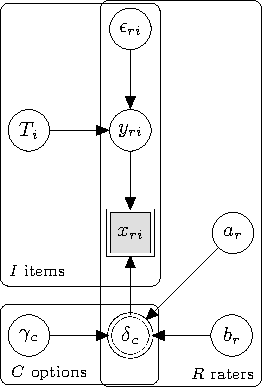
\includegraphics[width=.4\textwidth, page=1]{graphicalModels/graphicalModels.pdf}
	\caption{Graphical model corresponding to the CCT model for a single patient.}
	\label{model:CCTO}
\end{figure}

To formally introduce the CCT model for the ordinal case, the rating given by rater $\Irater$ on item $\Iitem$ is denoted $x_{\Irater\Iitem}$, and can take on discrete values from $1$ through $\Tncat$. %The discrete outcomes are the result of categorizing a continuous appraisal $y_{\Iitem\Irater}$ using a set of thresholds $\delta_{\Irater\Incat}$. 
The realization of $x_{\Iitem\Irater}$ is assumed to follow an ordered logistic distribution\footnote{The choice for an ordered logistic distribution is arbitrary and an ordered probit distribution could also be used.} with location $y_{\Iitem\Irater}$ and thresholds $\delta_{\Irater\Incat}$:

\begin{align*}
%\text{OrderedLogistic}
P(x_{\Iitem\Irater}\mid y_{\Iitem\Irater},\delta_{\Irater}) = 
\left\{\begin{array}{ll} 
	1 - \ilogit{(y_{\Iitem\Irater} - \delta_{\Irater 1}}         & \text{if } x_{\Iitem\Irater} = 1, \\[4pt]
	\ilogit{y_{\Iitem\Irater} - \delta_{\Irater,\Incat-1}} - 
	\ilogit{y_{\Iitem\Irater} - \delta_{\Irater,\Incat}}         & \text{if } 1 < x_{\Iitem\Irater} < \Tncat,\\[4pt]
	\ilogit{y_{\Iitem\Irater} - \delta_{\Irater,\Tncat-1}}       & \text{if } x_{\Iitem\Irater} = \Tncat. 
\end{array} \right.
\end{align*}
The ordered logistic distribution uses $\Tncat - 1$ thresholds to assign each of the $\Tncat$ outcomes a probability. This probability is equal to the area between subsequent thresholds for a logistic distribution, as illustrated in Figure~\ref{fig:orderedLogistic}.
\begin{figure}
	\centering
	\begin{subfigure}{.5\textwidth}
		\centering
		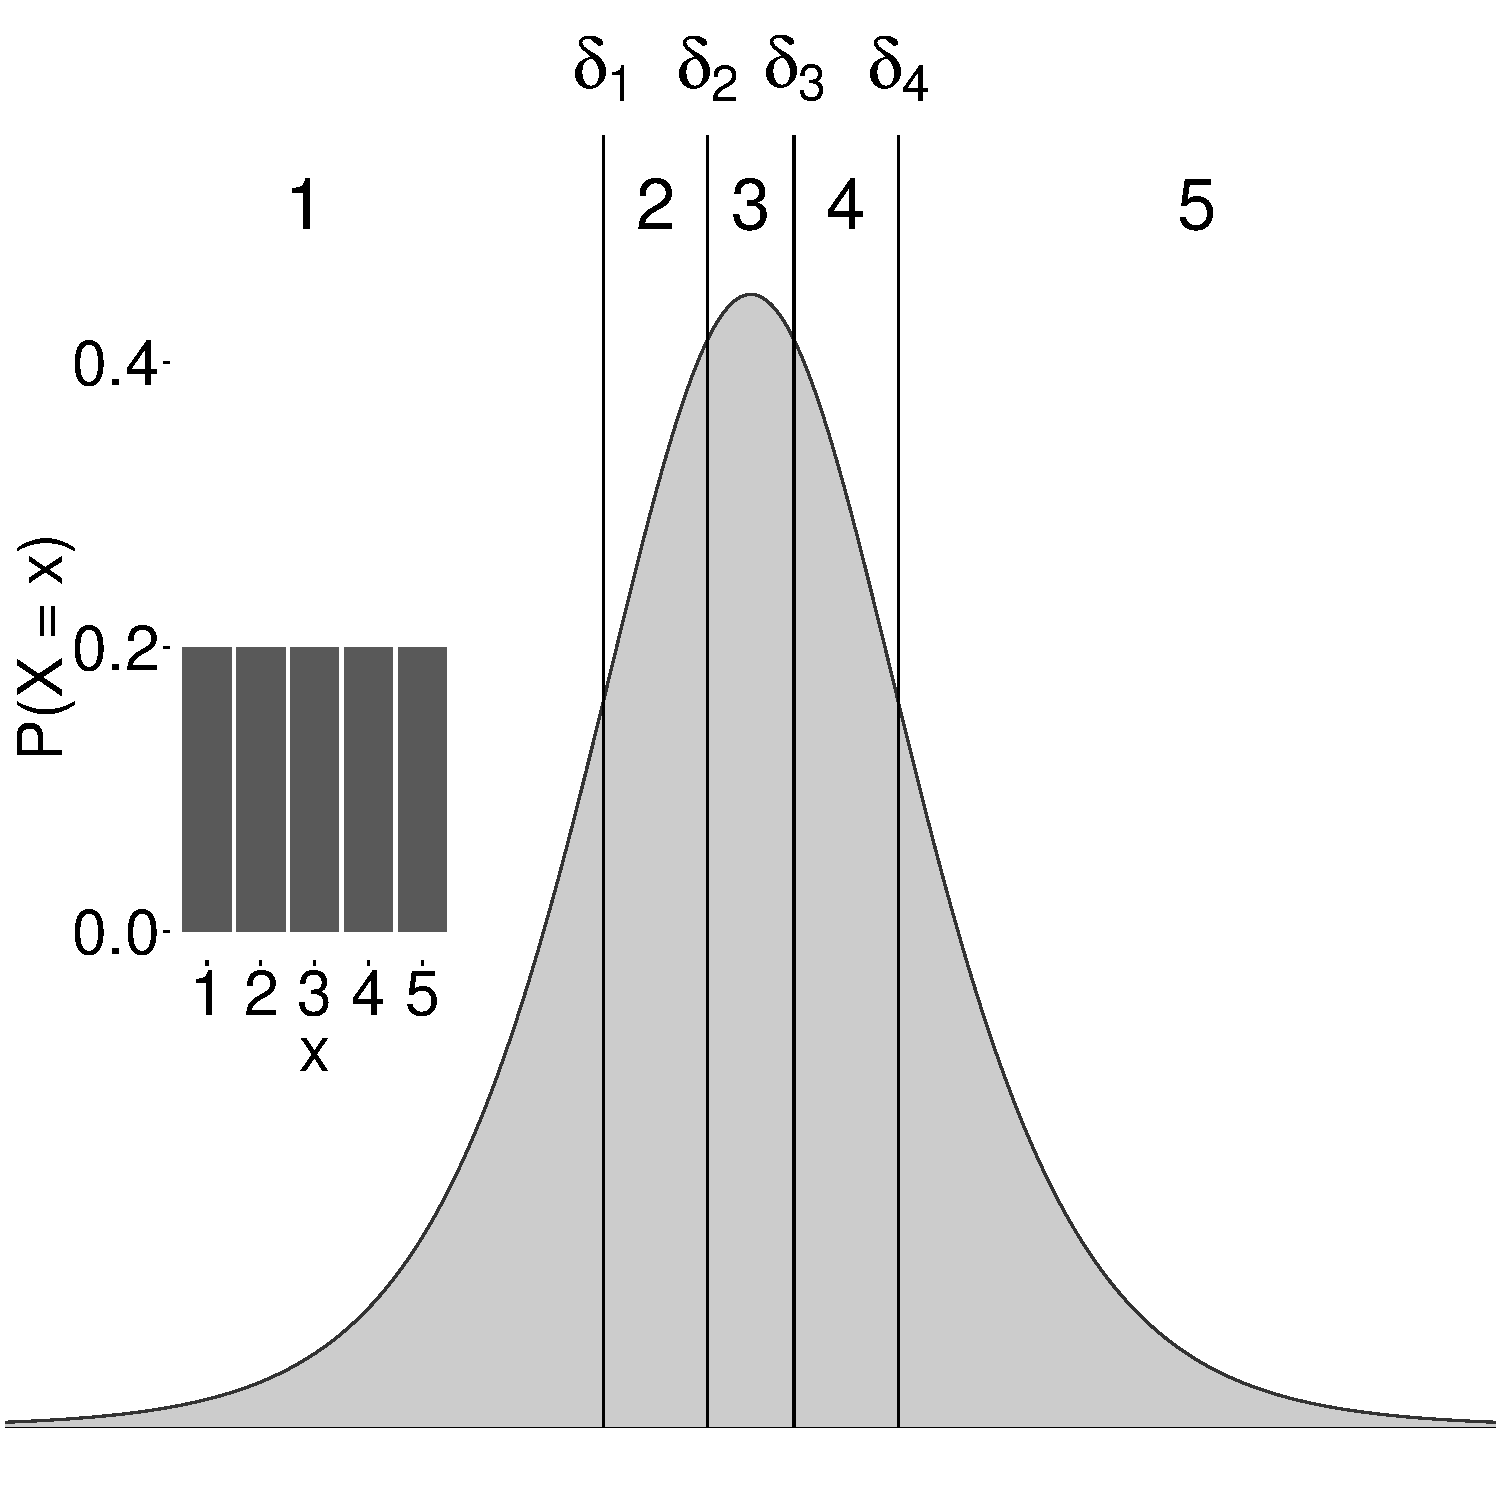
\includegraphics[width=\linewidth]{figures/orderedLogisticUnbiased.pdf}
%		\caption{A subfigure}
%		\label{fig:sub1}
	\end{subfigure}%
	\begin{subfigure}{.5\textwidth}
		\centering
		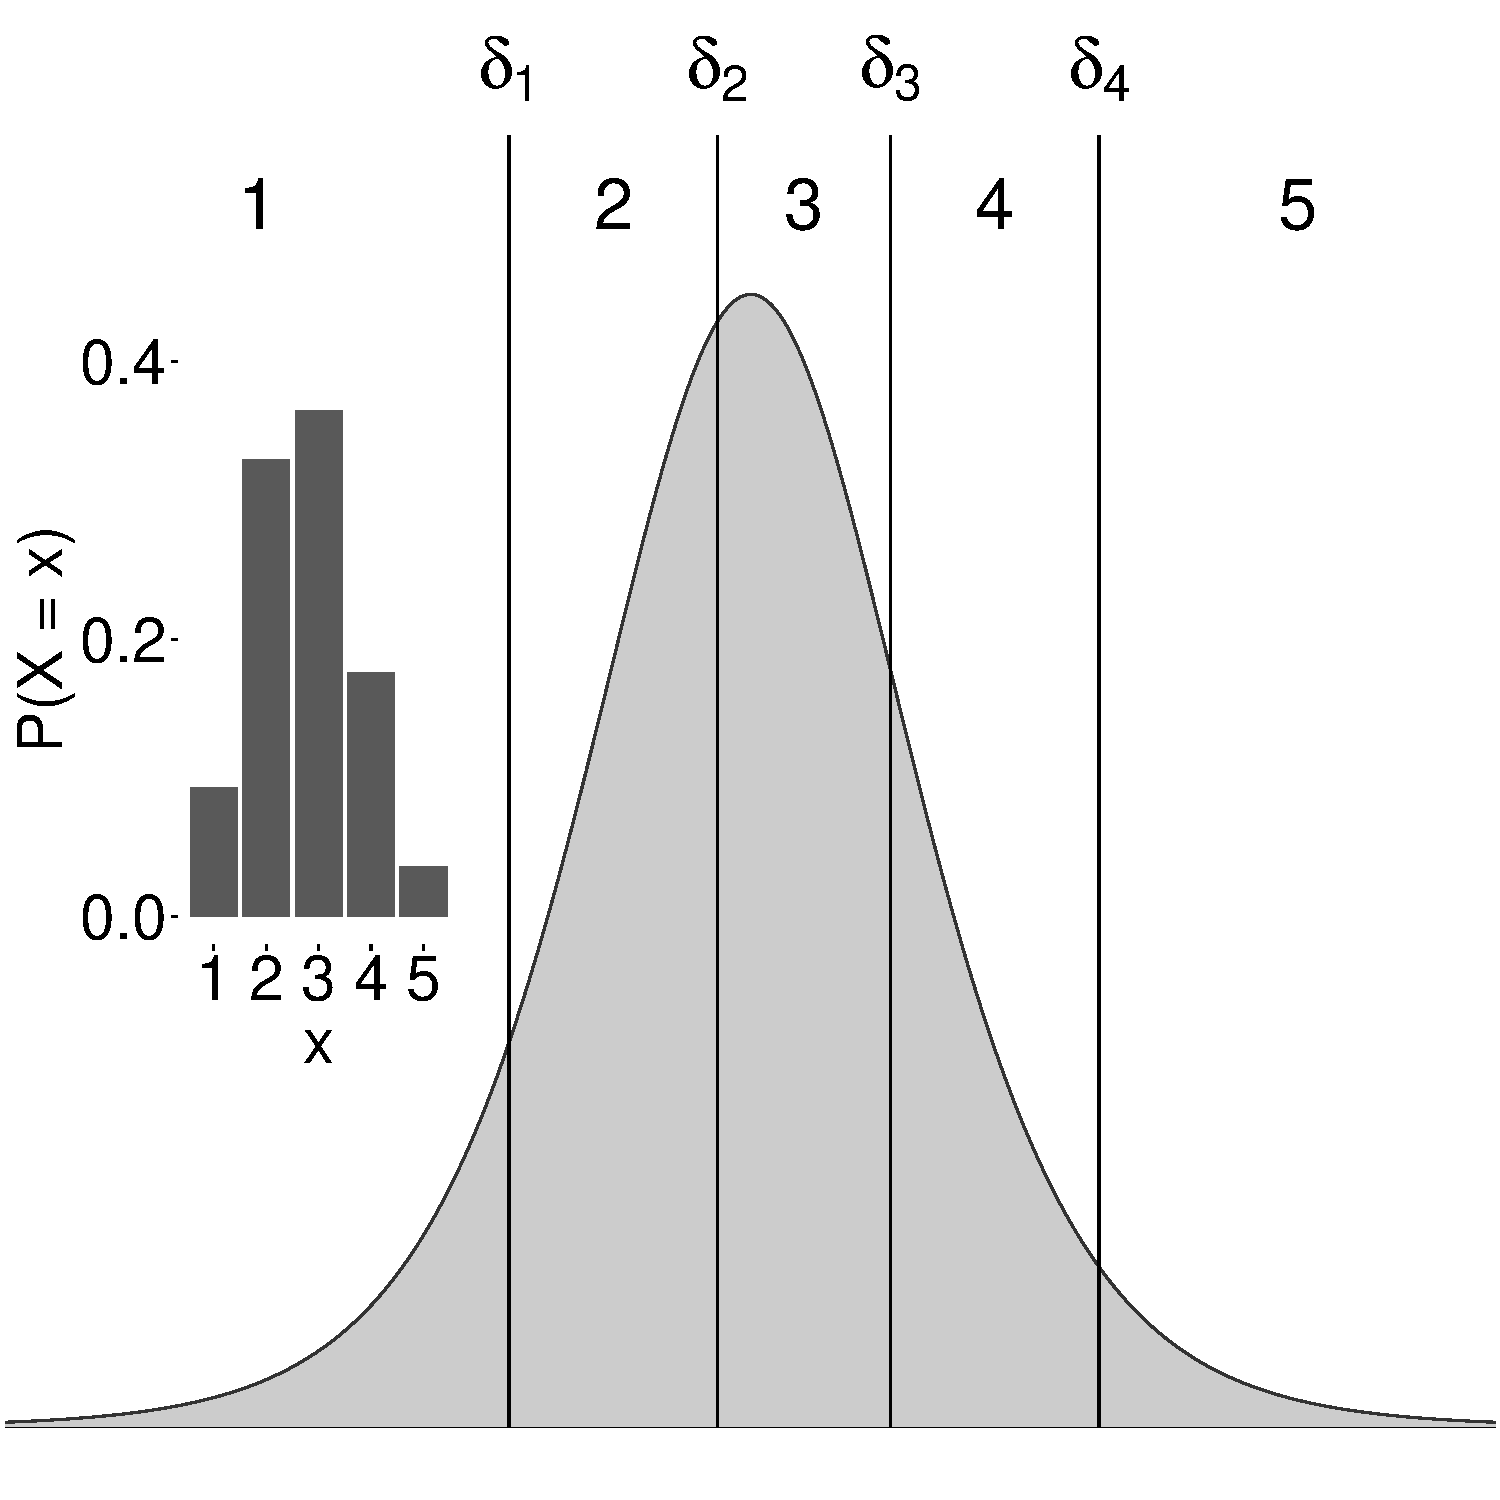
\includegraphics[width=\linewidth]{figures/orderedLogisticBiased.pdf}
%		\caption{A subfigure}
%		\label{fig:sub2}
	\end{subfigure}
	\caption{Ordered Logistic Distribution for $y_{\Iitem\Irater} = 0$ and varying thresholds. The implied probability distribution over categories is shown inside each panel. In the left panel, the thresholds are unbiased, $\alpha_\Irater = 1$, $\beta_\Irater = 0$. As a consequence, the distribution over outcomes is uniform. In the right panel, the thresholds are shifted right and the scale increased slightly, $\alpha_\Irater = 2$, $\beta_\Irater = 0.5$. The distribution over outcomes has most mass on outcomes 2 and 3.}
	\label{fig:orderedLogistic}
\end{figure}
\DON{Als ik zo naar het model kijk vraag ik me af waarom we de bias in de latent appraisal nodig hebben, en of deze niet al opgevangen wordt door de rater specifieke thresholds.} The main purpose of the ordered logistic distribution is to translate each observed rating into some latent appraisal score $y_{\Iitem\Irater}$ which can subsequently be linked to patient, rater, and item characteristics. 
The model contains two components that can capture rater bias. First, the appraisal of a rater for a given item can be biased. Therefore the appraisal is the sum of two components, the true score for an item $T_\Iitem$ and the bias of the rater $\epsilon_\Irater$. This captures that ..., Second, the  thresholds are allowed to differ across raters. An initial guess for the thresholds is $\ilogit{c/C}$. This yields a set of thresholds such that if the latent appraisal is 0 then $P(x_{\Iitem\Irater})$ is uniform.

Starting from an initial guess that the thresholds are distributed uniformly over the logistic distribution (here uniformly means, i.e., the ), 

Rather than modeling each of the $\Tncat - 1$ thresholds individually, the thresholds are modeled as a deviation from an unbiased set of thresholds. The thresholds are obtained by shifting and rescaling an unbiased threshold placement to estimate a potentially large number of thresholds instead of needing a parameter per threshold \cite{Fox1995, Gonzalez1999}.

vary across raters. Rather than modeling each of the $\Tncat - 1$ thresholds individually, we adopt the approach to 

The thresholds are obtained by shifting and rescaling an unbiased threshold placement to estimate a potentially large number of thresholds instead of needing a parameter per threshold \cite{Fox1995, Gonzalez1999}.

 

The appraisals consists of the latent truth $T_\Iitem$ for each item and the bias of each rater $\epsilon_\Irater$. The thresholds are obtained by shifting and rescaleing 


to estimate a potentially large number of thresholds instead of needing a parameter per threshold \cite{Fox1995, Gonzalez1999}.


\newpage


personen/ raters zijn gebiased. Kan niet alleen eigenschappen van de gedetineerden halen maar ook die van de raters.

Covariaat voor e.g., hulpverleners versus psychiaters. Meerdere groepen raters (fixed effect).

Hierachisch niveau over patienten.

Covariaat voor groepen gedetineerden (fixed effect misdrijf).
Ofwel order restrictie voor deze groepen.

Missing values?

Hoe combineren we verschillende schalen van items?

kaart van hoe ontwikkelt zich dit over de tijd (zie figuur in proposal)

TODO: change model in NWO proposal to mimic SDT approach.

Data is simulated using R \cite{R} and the posterior distributions are sampled from using Stan \cite{CarpenterEtAl2017Stan}.

\section*{Simulation Results}


\section*{Discussion}


A common application of CCT is testing for multiple consensus truths.

\subsection*{Limitations}

Aanbeveling voor de praktijk

Bijhouden van evaluaties (scores + rater), liefst met hoge frequentie. 
Reden waarom iemand opgesloten is (reason of incarceration).
zo min mogelijk missing not at random.
``handig'': training in invullen om verschillen tussen raters te minimalizeren.
(V)AR component?

\bibliographystyle{apacite}
\bibliography{references}

\end{document}
